\documentclass[12pt]{article}
\usepackage{CJKutf8}
\usepackage{geometry}
\usepackage{listings}
\usepackage{amsmath}
\usepackage{commath}
\usepackage{graphicx}

\lstset{frame=tb,
    language=Matlab}

\newgeometry{vmargin={6mm,10mm}, hmargin={10mm,10mm}}   
\begin{CJK}{UTF8}{bsmi}
\author{b05502087 王竑睿}
\date{}
\title{數值線性代數 HW4}

\begin{document}
\maketitle
\section{Let A be a 2 × 2 matrix of the form}
    \[
    A=
    \left[ 
        \begin{array}{cc}
        1 & 2\\
        3 & 4\\
        \end{array} 
    \right]
    \]
    \subsection*{Find an orthogonal 2 × 2 matrix Q such that $T = Q^TAQ$ is an upper triangular
    matrix; derive Q step by step}
    \subsection*{[solution:]}
    \begin{itemize}
        \item 先計算A的兩個特徵值$\lambda_1, \lambda_2$
            \[
                \begin{aligned}
                        &det(A-\lambda I)=0\\
            \Rightarrow &(1-\lambda)(4-\lambda)-6 = 0
            \Rightarrow \lambda_1 = \frac{-\sqrt{33}+5}{2}, \quad \lambda_2 = \frac{\sqrt{33}+5}{2}
                \end{aligned}
            \]
        \item 求出A的特徵向量$v_1, v_2$
            \[  
                \begin{aligned}
                        &(A-\lambda_1 I)v=0\\
            \Rightarrow &v1 = \left(
                                \begin{array}{c}
                                    \dfrac{-\sqrt{33}-3}{6}\\
                                    1
                                \end{array}
                            \right)
                \end{aligned}
            \]
            \[
                \begin{aligned}
                    &(A-\lambda_2 I)v=0\\
            \Rightarrow &v2 = \left(
                            \begin{array}{c}
                                \dfrac{\sqrt{33}-3}{6}\\
                                1
                            \end{array}
                        \right)
                \end{aligned}
            \]
        \item 將兩個特徵向量作 gram schmidt 得到 $e_1, e_2$
            \[  
                e_1=
                \begin{aligned}
                    v_1=\left(
                        \begin{array}{c}
                            \dfrac{-\sqrt{33}-3}{6}\\
                            1
                        \end{array}
                    \right)
                \end{aligned}
            \]
            \[
                \begin{aligned}
                    e_2 &= v_2-\frac{v_2 \cdot v_1}{v_1 \cdot v_1} v_1
                        &= \left(
                            \begin{array}{c}
                                \dfrac{\sqrt{33}-3}{6}\\
                                1
                            \end{array}
                        \right)
                \end{aligned}
            \]
        \item 將$e_1, e_2$化為orthonormal 得到 $q_1, q_2$
            \[  
                \begin{aligned}
                    q_1 &=\dfrac{e_1}{\norm{e_1}_2}\\
                        &=\left(
                        \begin{array}{c}
                            -\dfrac{\sqrt{6}+\sqrt{22}}{2\sqrt{\sqrt{33}+13}}\\
                            \dfrac{\sqrt{6}}{\sqrt{\sqrt{33}+13}}
                        \end{array}
                    \right)
                \end{aligned}
            \]
            \[
                \begin{aligned}
                    q_2 &=\dfrac{e_2}{\norm{e_2}_2}\\
                        &=\left(
                        \begin{array}{c}
                            \dfrac{\sqrt{187}(-33+13\sqrt{33})}{374\sqrt{13-\sqrt{33}}}\\
                            \dfrac{\sqrt{187}(\sqrt{33}+55)}{374\sqrt{13-\sqrt{33}}}\\
                        \end{array}
                    \right)
                \end{aligned}    
            \]
        \item $Q = [q_1, q_2]$
            \[
                \begin{aligned}
                    Q&=\left(
                        \begin{array}{cc}
                            -\dfrac{\sqrt{6}+\sqrt{22}}{2\sqrt{\sqrt{33}+13}}&\dfrac{\sqrt{187}(-33+13\sqrt{33})}{374\sqrt{13-\sqrt{33}}}\\
                            \dfrac{\sqrt{6}}{\sqrt{\sqrt{33}+13}}&\dfrac{\sqrt{187}(\sqrt{33}+55)}{374\sqrt{13-\sqrt{33}}}\\
                        \end{array}
                    \right)
                \end{aligned}    
            \]
    \end{itemize}
    \textbf{使用 matlab 計算 $Q^TAQ$ 的結果}\\
    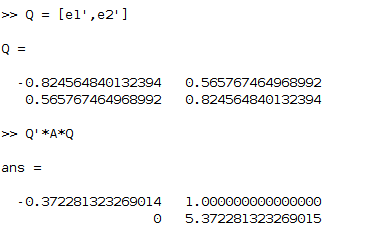
\includegraphics[scale=1]{schur.png}\\
    \textbf{$Q^TAQ$確實為上三角矩陣}
\section{Let $\lambda$ be a simple eigenvalue of A $\in$ $R^{m \times m}$ with right eigenvector x and left
eigenvector y (that is, Ax = $\lambda$x and yA = y$\lambda$), normalized so that $\norm{x}_2$ = $\norm{y}_2$ = 1. Define the eigenvalue condition number by $\kappa(\lambda, A) = 1/|y*x|$.}
\subsection*{(a)}
    \subsection*{[solution:]}
    \[
        \begin{aligned}
                &(A+\delta A)(x+\delta x) = (\lambda + \delta \lambda)(x+\delta x)\\
    \Rightarrow & Ax + A\delta x + \delta A x +\delta A\delta x = \lambda x + \lambda \delta x +\delta \lambda x + \delta \lambda \delta x\\
    \Rightarrow & A\delta x + \delta A x = \lambda \delta x +\delta \lambda x + (\delta \lambda \delta x - \delta A\delta x) \quad \text{(因為$Ax=\lambda x$)}\\ 
    \Rightarrow & (A-\lambda I)\delta x + \delta A x = \delta \lambda x + (\delta \lambda \delta x - \delta A\delta x)\\
    \Rightarrow & y^*(A-\lambda I)\delta x + y^*\delta A x = \delta \lambda y^*x + y^*(\delta \lambda \delta x - \delta A\delta x)\\
    \Rightarrow & 0 + y^*\delta A x = \delta \lambda y^*x + y^*(\delta \lambda \delta x - \delta A\delta x) \quad \text{(因為y是A的left eigenvector)}\\ 
    \Rightarrow & y^*\delta A x  + y^*(\delta A\delta x - \delta \lambda \delta x)= \delta \lambda y^*x\\ 
    \Rightarrow & \delta \lambda = \frac{y^*\delta A x}{y^*x}  + \frac{y^*(\delta A\delta x - \delta \lambda \delta x)}{y^*x}\\
    \Rightarrow & \delta \lambda = \frac{y^*\delta A x}{y^*x}  + O(\norm{\delta A}_2\norm{\delta x}_2)\\ 
    \Rightarrow & \delta \lambda = \frac{y^*\delta A x}{y^*x}  + O(\norm{\delta A}_2^2) \quad \text{(由power method $\norm{\delta x}_2 = O(\norm{\delta A}_2)$)}\\ 
        \end{aligned}
    \]
\subsection*{Demonstrate the sensitivity of $\lambda$ with a simple example for m = 16, for instance.}
下圖為random產生16$\times$16的矩陣所demo出的sensitivity of $\lambda$\\
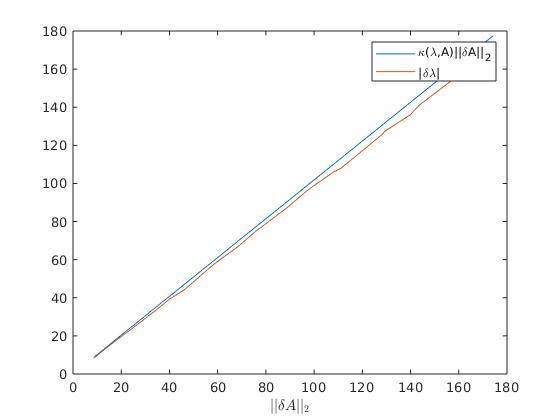
\includegraphics[scale = 0.75]{random_demo.jpg}

\subsection*{(b)}
\subsection*{[solution:]}
    \begin{itemize}
        \item calculate the eigenvalue of the Jordan Block
            \[
                \begin{aligned}
                        &det(J- \lambda_h I) = 0\\
            \Rightarrow &(\lambda-\lambda_h)^m = 0\\
            \Rightarrow &\lambda_h = \lambda\\
                \end{aligned}
            \]
        \item calculate the right eigenvector of the Jordan Block
            \[
                \begin{aligned}
                        &(J- \lambda I)x = 0\\
            \Rightarrow &   \left[\begin{array}{cccc}
                                0 & 1       \\
                                  & 0 & 1        \\
                                  &\ddots& \ddots  & 1 \\
                                  &      & \hdots  & 0 \\
                            \end{array}\right]x = 0\\
            \Rightarrow &   x = span(\left[\begin{array}{c}
                                                1\\
                                                0\\
                                                \vdots\\
                                                0\\
                                            \end{array}
                                        \right])\\
                \end{aligned}
            \]
        \item calculate the left eigenvector of the Jordan Block
            \[
                \begin{aligned}
                        &y(J- \lambda I) = 0\\
            \Rightarrow &(J- \lambda I)^Ty^T = 0\\
            \Rightarrow &   \left[\begin{array}{cccc}
                                0 &             \\
                                1 & 0 & \ddots  & \\
                                  & \ddots  &  0 & \\
                                  &   &  1 & 0 \\
                            \end{array}\right]y^T = 0\\
            \Rightarrow &   y^T = span(\left[\begin{array}{c}
                                                0\\
                                                0\\
                                                \vdots\\
                                                1\\
                                            \end{array}
                                        \right])\\
            \Rightarrow &   y = span([0,0,\hdots,1])\\
                \end{aligned}
            \]
        \item calculate the eigenvalue condition number
            \[
                \begin{aligned}
                        & \kappa(\lambda,J)\\
                    =   & 1/\abs{y^*x}\\
                    =   & \infty \quad \text{(因為 $y^*x = 0$)} \\
                \end{aligned}    
            \]
    \end{itemize}
    \subsection*{Demonstrate the sensitivity of $\lambda$ with a simple example for m = 16, for instance.}
        下圖為產生16$\times$16的Jordan-Block矩陣所demo出的sensitivity of $\lambda$\\
        由於$\kappa(\lambda,A)$為$\infty$,所以$\kappa(\lambda,A)\norm{\delta A}_2$未出現在圖中\\
        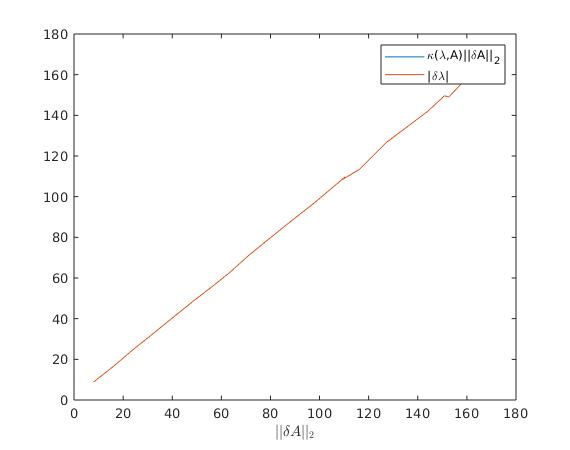
\includegraphics[scale = 0.75]{Jordan_demo.jpg}\\
此兩項Demo是利用以下code產生matrix,計算sensitivity,畫圖得到
\begin{lstlisting}
    function generate_matrix(m)
        J = zeros(m,m);
        la = 3;
        for i = 1:m
            for j = 1:m
                if(i==j)
                    J(i,j)=la;
                elseif(i==(j-1))
                    J(i,j)=1;
                end
            end
        end
        J
        Calculate_sense(J)
        A = rand(m,m);
        Calculate_sense(A);
    end
    function Calculate_sense(A)
        [lambda,x,y]=getxy(A);
        Y_delta_lambda = []
        Y_delta_A = []
        X_norm = []
        for len = 1:20
            delta_A = len*rand(16,16);
            A_plus_delta = A+delta_A;

            kappa = 1 / abs(y*x);
            delta_A_norm = norm(delta_A);
            X_norm = [X_norm, delta_A_norm];

            [lambda_2,x_2,y_2]=getxy(A_plus_delta);
            delta_lambda = abs(lambda_2-lambda);

            Y_delta_lambda = [Y_delta_lambda,delta_lambda];
            Y_delta_A = [Y_delta_A,kappa*delta_A_norm];
        end
        figure();
        plot(X_norm,Y_delta_A);
        hold on
        plot(X_norm,Y_delta_lambda)
        legend("\kappa(\lambda,A)||\deltaA||_2","|\delta\lambda|",'latex')
        xlabel("$||\delta A||_2$",'interpreter','latex');

        X_norm
        Y_delta_lambda
        Y_delta_A
        
    end
    function [lambda,x,y]=getxy(A)
        [Vr,Dr] = eig(A);
        [Vl,Dl] = eig(A');
        Dr(1,1);
        Vr(:,1);
        Dl(1,1);
        Vl(:,1);

        x = Vr(:,1);
        y = Vl(:,1)';
        lambda = Dr(1,1);
    end
\end{lstlisting}
    \section{Let $\hat T$ and T be two m $\times$ m tridiagonal toeplitz matrices of the form}
            \[
                \hat T =
                \left[
                \begin{array}{cccc}
                0 & 1   \\
                1 & \ddots & \ddots & \\
                  & \ddots & \ddots & 1\\
                  &        &    1   & 0\\
                \end{array}\right]
                ,
                T =
                \left[
                \begin{array}{cccc}
                a & b   \\
                b & \ddots & \ddots & \\
                  & \ddots & \ddots & b\\
                  &        &    b   & a\\
                \end{array}\right]
            \]
        \subsection*{(a) Show that the eigenvalues and the corresponding eigenvectors are}
                \[
                    \lambda_j=2cos(\dfrac{j \pi}{m+1}), 
                    v_j = \left[\begin{array}{c}
                            sin(\dfrac{j \pi}{m+1})\\
                            sin(\dfrac{2j \pi}{m+1})\\
                            \hdots\\
                            sin(\dfrac{mj \pi}{m+1})\\
                            \end{array}\right]
                \]
                ,where $\hat Tv_j = \lambda_jv_j$, for j = 1, 2,...,m.
        \subsection*{[solution:]}
                \begin{itemize}
                    \item Calculate eigenvalues
                        \[
                            \begin{aligned}
                                &det(\hat{T}-\lambda I)=0\\
                    \Rightarrow &det(T^h)=0 \quad \text{(令 $T^h$ 為 $\hat{T}-\lambda I$)}\\
                                &det(T^h_m)=(-\lambda)det(T^h_{m-1})+(-1)det(T^h_{m-2}) \quad \text{(由行列式降階, $T^h_m$表示取$T^h$的左上角$m \times m$部份)}\\
    &\text{令$-\lambda=2x$,} \\
    &\text{由chebyshev polynomial知$det(T^h_m)$是一個x的m次多項式,且m個root為}\\
                                &x_k = cos(k\pi/(m+1)), k=1,2,...,m\\
    &\text{轉換回$\lambda$形式的root}\\
                                &\lambda_k = (-2)cos(k\pi/(m+1)), k=1,2,...,m\\
    &\text{由於cos對角度有互補會差一個負號}\\
                                & \lambda_k = (-2)cos(k\pi/(m+1)) = 2cos((m+1-k)\pi/(m+1)) = (-1)\lambda_{m+1-k}, k=1,2,...,m\\
    &\text{因此,上述式子也可以去除負號}\\
                                &\lambda_k = 2cos(k\pi/(m+1)), k=1,2,...,m\\
                            \end{aligned}
                        \]
                        \text{所以}\\
                                $$\lambda_j = 2cos(j\pi/(m+1)), j=1,2,...,m$$\\
                    \item Calculate corresponding eigenvectors 
                        \[
                            \begin{aligned}
                                &\text{若有$\lambda_j = 2cos(j\pi/(m+1)), j=1,2,...,m$}\\
                                &\text{令$\theta_j = \frac{j\pi}{m+1}$, $v_{jk}$為$v_j$的第k個element, 證明:$v_{jk} = sin(k\theta_j)$}\\
                                &\text{使用數學歸納法}\\
                                &k=1: \text{we normalize the eigenvector with making its first element become } sin(\theta)\\
                                &k=2:\\
                                    & \quad \text{從$\hat{T}v_j=\lambda_jv_j$, 可以得到$v_{j2} = \lambda_j v_{j1}$}\\
                                    & \quad \quad v_{j2} = 2cos(j\pi/(m+1))sin(\theta) = 2cos(\theta)sin(\theta) = sin(2\theta)\\
                                &\text{假設$k = k'-1, k'-2$時, $v_{jk} = sin(k\theta_j)$皆成立,則}\\
                                &k=k':\\
                                    & \quad \text{從$\hat{T}v_j=\lambda_jv_j$, 可以得到}\\
                        \Rightarrow & v_{jk'} = \lambda_j v_{j(k'-1)}}-v_{j(k'-2)\\
                        \Rightarrow & v_{jk'} = \lambda_j sin((k'-1)\theta)-sin((k'-2)\theta)\\
                        \Rightarrow & v_{jk'} = 2cos(\theta)sin((k'-1)\theta)-sin((k'-2)\theta)\\
                        \Rightarrow & v_{jk'} = sin(k'\theta) \quad \text{(由 chebyshev polynomial)}
                        \Rightarrow \text{k=k'時,亦成立}\\
                        \text{所以}\\
                                &v_j = \left[\begin{array}{c}
                                    sin(\theta_j)\\
                                    sin(2\theta_j)\\
                                    \hdots\\
                                    sin(m\theta_j)\\
                                    \end{array}\right]
                                     = \left[\begin{array}{c}
                                        sin(\dfrac{j \pi}{m+1})\\
                                        sin(\dfrac{2j \pi}{m+1})\\
                                        \hdots\\
                                        sin(\dfrac{mj \pi}{m+1})\\
                                        \end{array}\right]
                            \end{aligned}
                        \]
                \end{itemize}
        \subsection*{(b) What are the eigenvalues of T?}
        \subsection*{[solution:]}
        令$\lambda^{\hat{T}}_{j}$為$\hat{T}$的第j個eigenvalue\\
        \[
            \begin{aligned}
                &\text{由於 $T = a+b\hat{T}$}\\
                \text{因此}&\\
                & \lambda^{\hat{T}}_{j} = a+b\lambda_{j}\\
    \Rightarrow & \lambda^{\hat{T}}_{j} = a+2bcos(j\pi/(m+1)), j=1,2,...,m\\
            \end{aligned}
        \]
        \text{所以}\\
                $$\lambda^{\hat{T}}_{j} = a+2bcos(j\pi/(m+1)), j=1,2,...,m$$\\
        \subsection*{(c) For m $=$ 32, plot the eigenvector of j $=$ 1, 2, 31, 32.}
        \subsection*{[solution:]}
        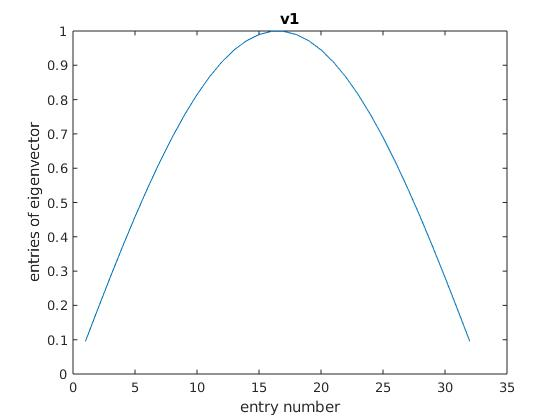
\includegraphics[scale=0.5]{v1.jpg}
        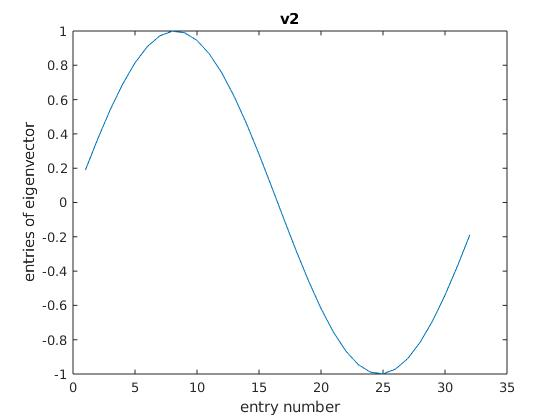
\includegraphics[scale=0.5]{v2.jpg}\\
        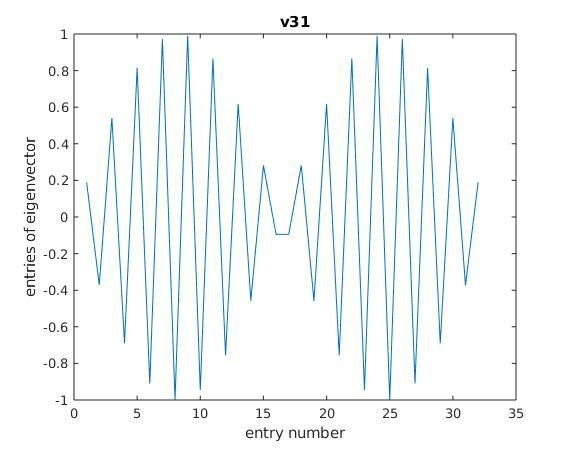
\includegraphics[scale=0.5]{v31.jpg}
        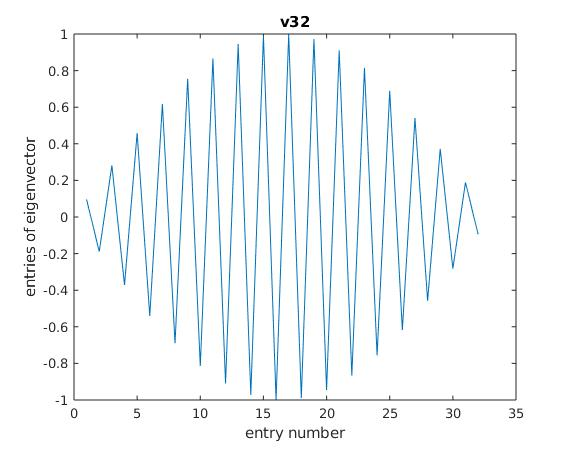
\includegraphics[scale=0.5]{v32.jpg}\\
    
    \section{Consider the matrix A written in Matlab as}
        \begin{lstlisting}
            A = diag(15:-1:1)+ones(15,1);
        \end{lstlisting}
        \subsection*{(a) Use the power iteration to find the largest eigenvalue of A. Comment on the
        rate of convergence of the method.}
        \subsection*{[solution:]}
        利用以下code,進行power Iteration
        \begin{lstlisting}
            function EigenValue = powerIter(A)
                [m,n] = size(A);
                x = rand(n,1);
                iterTime = 30;
                Y = [];
                [V,D] = eig(A);
                for i=1:iterTime
                    x = A*x;
                    x = x/norm(x);
                    x;
                    EigenValue = (x'*A*x) / (x'*x);
                    Y = [Y, EigenValue];
                end
                %eig(A)
                %EigenValue
                D(15,15);
                V(:,size(D,1));
                plot([1:iterTime],Y);
                xlabel("iterations")
                ylabel("estimated eigenvalue")
            end
        \end{lstlisting}
        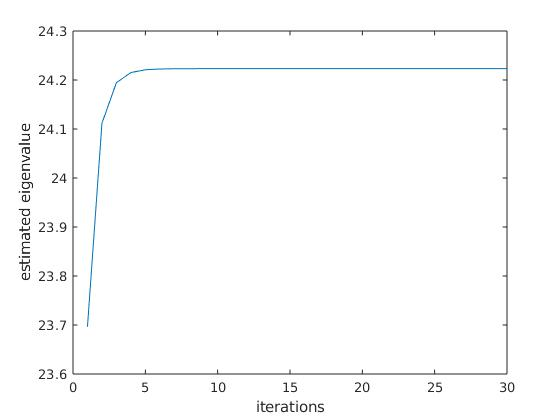
\includegraphics[scale=0.75]{powerIter.jpg}\\
        最大的eigenvalue為:24.2231\\
        大約花費了5個iteration達到收斂
        \subsection*{(b) Use the inverse iteration to find the eigenvector that corresponds to a selected
        eigenvalue. Comment on the rate of convergence of the method.}
        \subsection*{[solution:]}
        利用以下code,進行Inverse Iteration
        \begin{lstlisting}
            function EigenVector = InverseIter(A,mu)
                [m,n] = size(A);
                x = rand(n,1);
                iterTime = 30;

                [V,D] = eig(A);
                truth = V(:,size(D,1));
                Y = [];
                for i=1:iterTime
                    err = norm(abs(x)-abs(truth),2);
                    Y = [Y,err];
                    x = inv(A-mu*eye(m))*x;
                    x = x/norm(x);
                end
                EigenVector = x;
                plot([1:iterTime],Y);
                xlabel("iterations")
                ylabel("2-norm of error vector")
            end
        \end{lstlisting}
        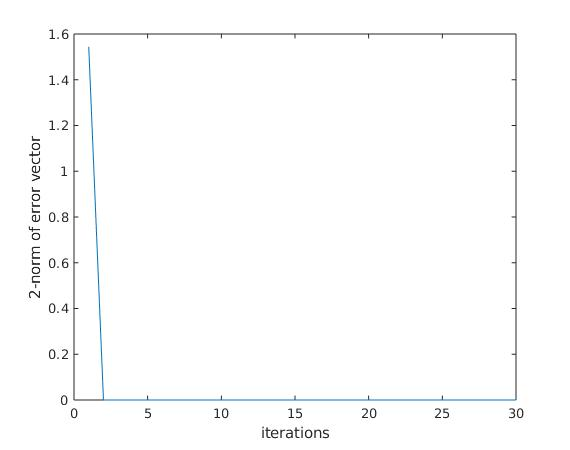
\includegraphics[scale=0.75]{inverseIter.jpg}\\
        選取的eigenvalue為(a)中求出的24.2231。
        對應的eigenvector為:
        \[\left[
            \begin{array}{c}
                0.4030\\
                0.3636\\
                0.3312\\
                0.3041\\
                0.2811\\
                0.2614\\
                0.2442\\
                0.2291\\
                0.2158\\
                0.2040\\
                0.1934\\
                0.1838\\
                0.1752\\
                0.1673\\
                0.1601
            \end{array}
        \right]\]
        大約2次iterations
        \subsection*{(c) Use the Rayleigh-quotient iteration to find the eigenvalue that corresponds to
        the eigenvector closest to the initial iteration vector. Comment on the rate of
        convergence of the method.}
        \subsection*{[solution:]}
        利用以下code,進行Rayleigh-quotient iteration
        \begin{lstlisting}
            function eigenValue = Rayleigh(A,b)
                [m,n] = size(A);
                iterTime = 100;
                mu = rand(1,1)
                Y = [mu];
                ct = 1;
                for i=1:iterTime
                    b = inv(A-mu*eye(m))*b;
                    mu2 = (b'*A*b) / (b'*b)
                    Y = [Y,mu2];
                    ct = ct+1;
                    if(norm(mu2-mu)<1e-10)
                        break;
                    end
                    mu = mu2
                end
                eigenValue = mu;
                Y
                plot([1:ct],Y);
                xlabel("iterations")
                ylabel("estimated eigenvalue")
                set(gca,'XTick',[1:1:ct])
            end
        \end{lstlisting}
        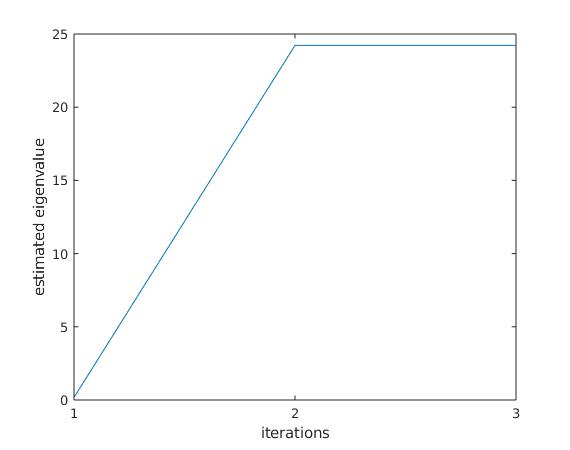
\includegraphics[scale=0.75]{Rayleigh.jpg}\\
        選取(b)所求出的eigenvector\\
        最大的eigenvalue為:24.2231\\
        幾乎是一次iteration就達到收斂
        \subsection*{(d) Use the "pure" QR iteration to find all the eigenvalues of A. In this case, plot
        the diagonal entries of a matrix undergoing QR iteration.}
        \subsection*{[solution:]}
        利用以下code,進行QRalgo
        \begin{lstlisting}
            function QRalgo(A,Thres,iterTime)
                %iterTime = 100;
                Toplot = [];
                it = 0;
                for i=1:iterTime
                    i
                    it = it + 1;
                    D = diag(A);
                    Toplot = [Toplot,D];
                    [Q,R] = qr(A);
                    A2 = Q'*A*Q;
                    if(norm(A2-A)<Thres)
                        break;
                    end
                    A = A2;
                end
                Toplot;
                figure();
                for i=1:15
                    plot([1:it],Toplot(i,[1:it]))
                    hold on
                end
                leg = string([1:15])
                for i=1:15
                    leg(i) = "entry" + leg(i);
                end
                legend(leg);
                xlabel("QR iterations");
                ylabel("diagonal entries");
                ret = diag(A)
            end
        \end{lstlisting}
        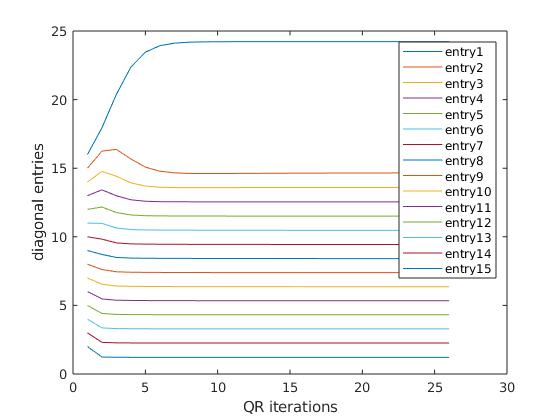
\includegraphics[scale=0.75]{entry.jpg}\\
        所有eigenvalue為:\[\left[
            \begin{array}{c}
                24.2231\\
                14.6589\\
                13.5912\\
                12.5415\\
                11.5020\\
                10.4687\\
                9.4392\\
                8.4124\\
                7.3872\\
                6.3630\\
                5.3390\\
                4.3143\\
                3.2878\\
                2.2570\\
                1.2147
            \end{array}
        \right]\]
        \subsection*{(e) Use the QR iteration with Wilkinson’s shift to find all the eigenvalues of A.}
        \subsection*{[solution:]}
        利用以下code,進行Wilkinson's shift
        \begin{lstlisting}
            function ret=WilkShift(A,Thres,iterTime)
                %iterTime = 100;
                [m,n] = size(A);
                I = eye(m);
                for i=1:iterTime
                    i
                    s = A(m,n);
                    [Q,R] = qr(A-s*I);
                    A2 = R*Q + s*I;
                    if(norm(A2-A)<Thres)
                        break;
                    end
                    A = A2;
                end
                ret = diag(A);
            end
        \end{lstlisting}
        所有eigenvalue為:\[\left[
            \begin{array}{c}
                24.2231\\
                14.6599\\
                13.5912\\
                12.5413\\
                11.5018\\
                10.4685\\
                9.4391\\
                8.4123\\
                7.3872\\
                6.3630\\
                5.3390\\
                4.3143\\
                3.2878\\
                2.2570\\
                1.2147
            \end{array}
        \right]\]
        \subsection*{(f) Discuss the rate of convergence of the QR method considered in (d) and (e).}
        \subsection*{[solution:]}
        利用以下code,比較QR iteration以及QR iteration with Wilkinson's shift在不同threshold下需要的iteration數
        \begin{lstlisting}
            function discuss(A)
                iterTime = 10^(9);
                Ywilk = [];
                YQR = [];
                for i = 1:10
                    Thres = 10^(-i);
                    [ret,TotalIter1]=WilkShift(A,Thres,iterTime);
                    [ret,TotalIter2]=QRalgo(A,Thres,iterTime);
                    Ywilk = [Ywilk,TotalIter1];
                    YQR = [YQR, TotalIter2];
                end
                figure();
                plot([1:10],Ywilk);
                %plot([10:10:100],Ywilk);
                hold on;
                plot([1:10],YQR);
                legend("QR iteration with Wilk shift","QR iteration");
                ylabel("iterations");
                xlabel("$-log_{10}(Threshold)$",'Interpreter','latex');
            end
        \end{lstlisting}
        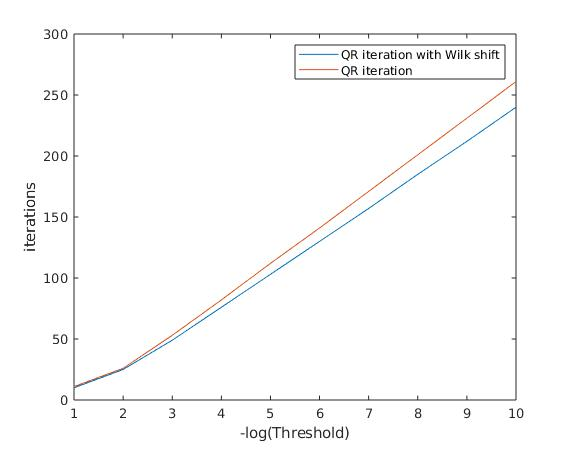
\includegraphics[scale=0.75]{discuss.jpg}\\
        \begin{itemize}
            \item 由圖可以看出,同樣的Threshold下,QR iteration with Wilkinson's shift都能比QR iterations用更少的iterations數收斂
        \end{itemize}
        
\end{CJK}
\end{document}